\documentclass[b5paper,papersize,dvipdfmx,fleqn]{jsarticle}
\usepackage{/Users/yamasakishun/Desktop/ymskarticle}
\usepackage{here}

\begin{document}
\title{理論演習II Essay}
\author{05-201564 Shun Yamasaki}
\date{\today}
\maketitle

\section{Abstract (200 words)}
線形連立一次方程式を解くことは周知の通り様々な場面で非常に重要な問題である。線形連立一次方程式は
\begin{eqnarray}
  A\vec{x} = \vec{b}
\end{eqnarray}
と表される。今回は,$\vec{x}$自体を知る必要はないが,ある行列$M$を用いて$\vec{x}^\dagger M \vec{x}$と表されるような$\vec{x}$に関係した量を求めたい場合を考える。$A$が行あたり最大$s$個のnon-zero成分を持つ$N\times N$の行列であり,条件数(condition number)\footnote{condition numberの説明を入れる}を$\kappa $とすると,知られている最速の古典アルゴリズムでは$\vec{x},\vec{x}^\dagger M \vec{x}$を計算するのに$N\sqrt{\kappa }$の時間スケールで計算できる。
一方,今回紹介する量子アルゴリズムでは$\vec{b}$に対応する状態$\ket{b}$が用意できた時,残りの$\vec{x}^\dagger M \vec{x}$を$\log(N),\kappa $ を求める計算ステップは多項式時間スケールで計算することができる。これは古典コンピュータに比べて指数関数的なスピードアップである。

\section{Introduction (1.5-2 pages)}
% \subsection{Quantum Computer}

量子コンピュータは量子力学を利用し,現状わかっている古典コンピュータによるアルゴリズムでは実現できない計算を含む計算を実現する装置である。Shorのアルゴリズムのように,ある特定の問題に対しては量子コンピュータは古典コンピュータよりはるかに早い時間で計算できる。この論文では線形連立一次方程式の解の特徴について考えていく。

% \subsection{Linear Equation}

線形方程式は科学技術・工学においてほぼ全ての分野で応用\footnote{「HHLから引用」と示す}され,非常に重要であると言える。古典コンピュータでは$N$次の線形方程式を解くのに,一般的に少なくとも$N$オーダーの時間がかかる。

% \subsection{Overview}

この論文では,特定の場合ではAbstractと同じ方程式
\begin{eqnarray}
  A\vec{x} = \vec{b}
\end{eqnarray}
において$A$が行あたり最大$s$個のnon-zero成分を持つ$N\times N$の行列であり,条件数(condition number)を$\kappa $とすると,解$\vec{x}$に関連した値を任意の精度で計算するのに$\log(N),\kappa $の多項式時間スケールかかるということを示している。これは古典コンピュータに比べて指数関数的なスピードアップである。また,典型的なケースでは正確性はあまり求められないことが多い。しかし,condition numberは計算量を著しく増大させ得る。これはこの論文におけるアルゴリズムにおける強い制約となっている。

上の線形方程式と同じ条件で以下,考えていくこととする。まず,$\vec{b}$は抽象的な状態$\ket{b}$の行列表現であると考える。$\vec{b}$と$\ket{b}$が必ずしも等価でないことに注意する。

% \subsection{Outline of the article}

以下では,
\begin{enumerate}
  \item algorithm(とruntime, comparison)
  \item このalgorithmがoptimalであると示す
  \item application
\end{enumerate}

% \subsection{related work}

また,related workとして制限付きでの線形操作の例や,非線形微分方程式への拡張の話題がある。

\section{Preliminary}
% これがないと下が読めないものを書く
\subsection{量子計算の基礎知識}
量子ビットは量子情報の入れ物の最小単位で,2準位基底では$\ket{0}, \ket{1}$を基底に取り一般の状態$\ket{\psi }$を$\ket{\psi }= \alpha \ket{0}+\beta \ket{1}$のように表すことが多い。ただし,$\alpha, \beta$は複素数の定数で,$|\alpha|^2 + |\beta|^2 = 1$である。

量子レジスタは異なるHilbert spaceに用意された量子ビットを複数並べたもので,ここではテンソル積を用いて$\ket{0}\otimes \ket{1}\otimes \cdots \otimes \ket{1}$のように表すものとする。

量子ゲートは量子レジスタに対する操作のことで,現在の主流な量子コンピュータでは数種類のunitary operatorの組み合わせ(これもunitary operatorになることが知られている)によって望みの状態を実現する。

量子回路は,量子レジスタにゲートを順番にかけていった回路図で,以下の図のように表される。
\begin{center}
  \begin{figure}[H]
    \centering
       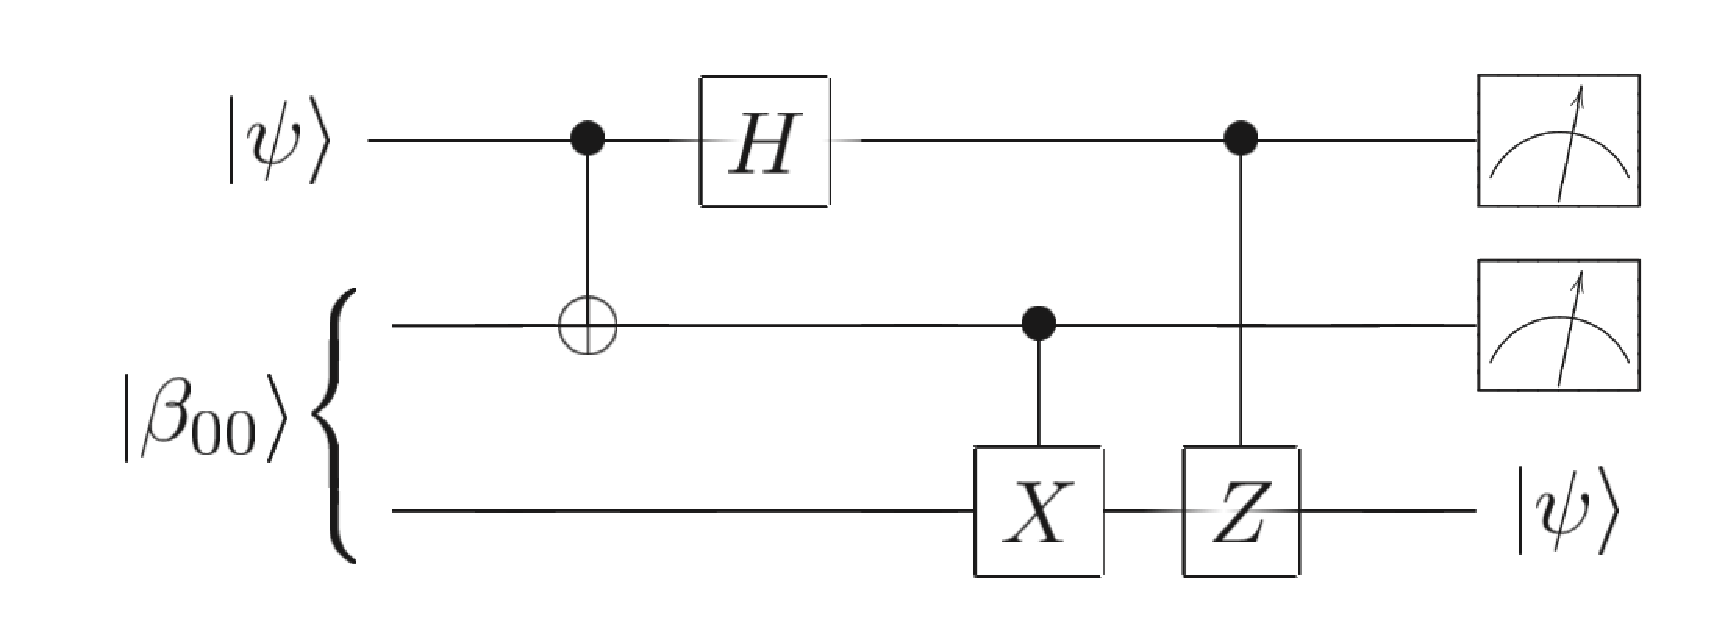
\includegraphics[width=0.5\textwidth]{circuit.pdf}
       \caption{quautum circuitの例(QCQIより引用)}
       \label{circuit}
  \end{figure}
\end{center}

measurementは終状態から情報を読みだす操作である。終状態 $\sum_{k=0}^{2^{n}-1} c_{k}|k\rangle$ から $p_{k}=\left|c_{k}\right|^{2}$を知ることを指し,回路の実行・測定を繰り返し,$0,1, \ldots, 2^{n_{-} 1}$ を得た回数を記録しヒストグラムから$\left\{p_{k}\right\}$を推定する。

\subsection{QFT}
QFT(Quantum Fourier transformation)は以下のように状態$\ket{j}$を変換する操作である。
$$
\begin{aligned}
|j\rangle & \rightarrow \frac{1}{2^{n / 2}} \sum_{k=0}^{2^{n}-1} e^{2 \pi i j k / 2^{n}}|k\rangle \\
&=\frac{1}{2^{n / 2}} \sum_{k_{1}=0}^{1} \cdots \sum_{k_{n}=0}^{1} e^{2 \pi i j\left(\sum_{l=1}^{n} k_{l} 2^{-l}\right)}\left|k_{1} \ldots k_{n}\right\rangle \\
&=\frac{1}{2^{n / 2}} \sum_{k_{1}=0}^{1} \cdots \sum_{k_{n}=0}^{1} \bigotimes_{l=1}^{n} e^{2 \pi i j k_{l} 2^{-l}}\left|k_{l}\right\rangle \\
&=\frac{1}{2^{n / 2}} \bigotimes_{l=1}^{n}\left[\sum_{k_{l}=0}^{1} e^{2 \pi i j k_{l} 2^{-l}}\left|k_{l}\right\rangle\right] \\
&=\frac{1}{2^{n / 2}} \bigotimes_{l=1}^{n}\left[|0\rangle+e^{2 \pi i j 2^{-l}}|1\rangle\right] \\
&=\frac{\left(|0\rangle+e^{2 \pi i 0 . j_{n}}|1\rangle\right)\left(|0\rangle+e^{2 \pi i 0 . j_{n-1} j_{n}}|1\rangle\right) \cdots\left(|0\rangle+e^{2 \pi i 0 . j_{1} j_{2} \cdots j_{n}}|1\rangle\right)}{2^{n / 2}} .
\end{aligned}
$$
% The product representation (5.4) makes it easy to derive an efficient circuit for the quantum Fourier transform. Such a circuit is shown in Figure 5.1. The gate $R_{k}$ denotes the unitary transformation
% $$
% R_{k} \equiv\left[\begin{array}{cc}
% 1 & 0 \\
% 0 & e^{2 \pi i / 2^{k}}
% \end{array}\right]
% $$
% To see that the pictured circuit computes the quantum Fourier transform, consider what happens when the state $\left|j_{1} \ldots j_{n}\right\rangle$ is input. Applying the Hadamard gate to the first bit produces the state
% $$
% \frac{1}{2^{1 / 2}}\left(|0\rangle+e^{2 \pi i 0 . j_{1}}|1\rangle\right)\left|j_{2} \ldots j_{n}\right\rangle
% $$
この計算は具体的に,以下のような回路で実現することができる。
\begin{center}
  \begin{figure}[H]
       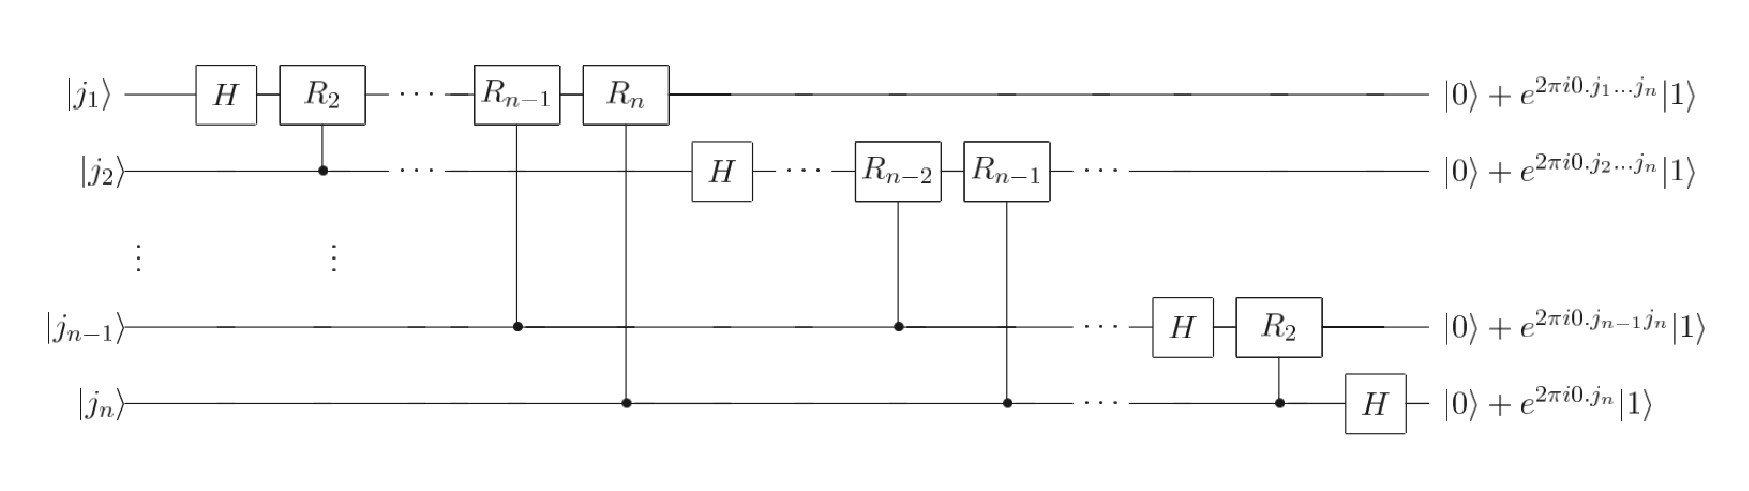
\includegraphics[width=\textwidth]{qft.pdf}
       \caption{QFTの例(QCQIより引用)}
       \label{circuit}
  \end{figure}
\end{center}
\subsection{QPE}
QPE(Quantum Phase Estimation)は位相を推定するためのアルゴリズムで,QFTを応用して計算する。具体的なアルゴリズムは以下の通りである。


Inputs:

 (1) A black box wich performs a controlled- $U^{j}$ operation, for integer $j$

 (2) an eigenstate $|u\rangle$ of $U$ with eigenvalue $e^{2 \pi i \varphi_{u}}$

 (3) $t=n+\left\lceil\log \left(2+\frac{1}{2 \epsilon}\right)\right\rceil$ qubits initialized to $|0\rangle$.


Outputs: An $n$-bit approximation $\widetilde{\varphi_{u}}$ to $\varphi_{u} .$


Runtime: $O\left(t^{2}\right)$ operations and one call to controlled- $U^{j}$ black box. Succeeds with probability at least $1-\epsilon$.


Procedure:


1. $|0\rangle|u\rangle$


2. $\quad \rightarrow \frac{1}{\sqrt{2^{t}}} \sum_{j=0}^{2^{t}-1}|j\rangle|u\rangle$ create superposition


3. $\rightarrow \frac{1}{\sqrt{2^{t}}} \sum_{j=0}^{2^{t}-1}|j\rangle U^{j}|u\rangle$ $=\frac{1}{\sqrt{2^{t}}} \sum_{j=0}^{2^{t}-1} e^{2 \pi i j \varphi_{u}}|j\rangle|u\rangle$ apply black box


4. $\quad \rightarrow\left|\widetilde{\varphi_{u}}\right\rangle|u\rangle$ apply inverse Fourier transform


5. $\rightarrow \widetilde{\varphi_{u}}$ measure first register

これを量子回路で実現すると以下のようになる。
\begin{center}
  \begin{figure}[H]
       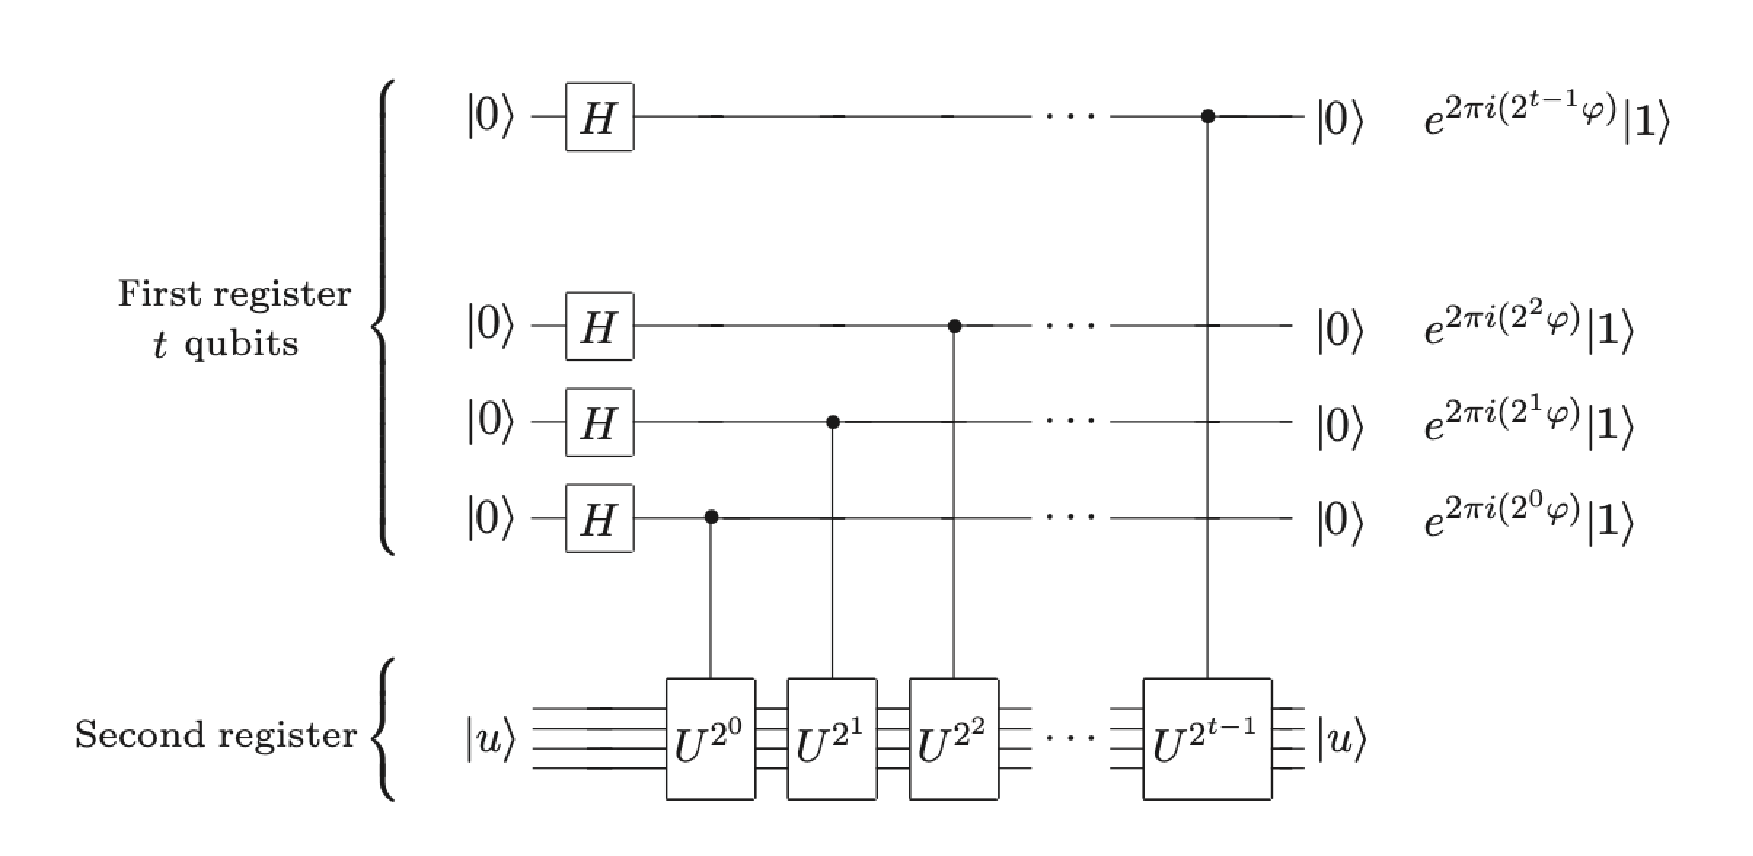
\includegraphics[width=\textwidth]{qpe.pdf}
       \caption{QPEの例(QCQIより引用)}
       \label{circuit}
  \end{figure}
\end{center}






\section{Main Result (1 page)}

具体的なアルゴリズムを紹介する。
\begin{enumerate}
  \item Ref[3]によって行列$A$を$e^{iAt}$に変換する。
  \item Ref[13]によって$\vec{b}$に対応する状態$\ket{b}$を用意する。
  \item 同様にRef[13]によって$\displaystyle \left|\Psi_{0}\right\rangle:=\sqrt{\frac{2}{T}} \sum_{\tau=0}^{T-1} \sin \frac{\pi\left(\tau+\frac{1}{2}\right)}{T}|\tau\rangle$なる状態$\left|\Psi_{0}\right\rangle$を用意する。
  \item $\displaystyle \sum_{\tau=0}^{T-1}|\tau\rangle\langle\tau| \otimes e^{i A \tau t_{0} / T}$ (unitary) on $\left|\Psi_{0}\right\rangle \otimes|b\rangle$, where $t_{0}=O(\kappa / \epsilon)$\footnote{epsilonの説明を入れる}のように用意した状態$\ket{b}$および$\left|\Psi_{0}\right\rangle$のテンソル積に対してconditional Hamiltonian evolutionを作用させる。
  \item first register(initial stateが$\left|\Psi_{0}\right\rangle$のregister)をFourier Transformationする。
  \item qubitを追加してrotationさせる。
  \item phase estimationをする。
  \item last qubitをmeasureする。
\end{enumerate}
以上のアルゴリズムによって,$\vec{x}$に関係した量を$\vec{b}$に対応する状態$\ket{b}$が用意できた時,残りの$\vec{x}^\dagger M \vec{x}$を$\log(N),\kappa $ を求める計算ステップは多項式時間スケールで計算することができる。



\section{Details, Discussion (2 page)}
以下ではMain Result で紹介したアルゴリズムがうまくいく理由について解説する。まず,Ref[3]で,行列$A$を$O(\log(N)s^2t)$をupper boundとする計算量で$\exp(iAt)$で計算することができる。

次に,行列$A$がHermitianかどうかで場合分けをする。

$A$がHermitianでない場合,
\begin{eqnarray}
  \tilde{A}:= \left(\begin{array}{cc}
0 & A \\
A^{\dagger} & 0
\end{array}\right)
\end{eqnarray}
と定義すれば$\tilde{A}$はHermitianであるので,方程式
$$
\tilde{A} \vec{y}=\left(\begin{array}{l}
\vec{b} \\
0
\end{array}\right)
$$
を解くことで
$$
\vec{y}=\left(\begin{array}{l}
0 \\
\vec{x}
\end{array}\right)
$$
が得られる。このように,$A$がHermitianでない時,$\tilde{A}$を定義して解けるようにする一連の操作をreductionと呼ぶ。

以下では,$A$がHermitianである場合を考える。Ref[13]により,$b_{i}$ and $\sum_{i=i_{1}}^{i_{2}}\left|b_{i}\right|^{2}$ are efficiently computableならstate $\ket{b}$を任意の基底における任意の確率振幅についての重ね合わせに変換できる。ここでは$\ket{b}$を$A$の固有ベクトル(単位ベクトルを選ぶ)をの重ね合わせで表すこととする。確率振幅には,$\vec{b}$の成分を割り当てることを考える。これでまた,$\left|u_{j}\right\rangle$をthe eigenvectors of $A$ , and $\lambda_{j}$をthe corresponding eigenvaluesとして,次を定義する。ここまでで$\ket{b}$が準備できた。

$$
\left|\Psi_{0}\right\rangle:=\sqrt{\frac{2}{T}} \sum_{\tau=0}^{T-1} \sin \frac{\pi\left(\tau+\frac{1}{2}\right)}{T}|\tau\rangle
$$

ただし,ここでは$T$は非常に大きな値とする。これで$
\left|\Psi_{0}\right\rangle$についても準備ができた。このようにして用意した$\ket{b}$および$\left|\Psi_{0}\right\rangle$のテンソル積に対してconditional Hamiltonian evolutionを作用させて

$\sum_{\tau=0}^{T-1}|\tau\rangle\langle\tau| \otimes e^{i A \tau t_{0} / T}$ (unitary) on $\left|\Psi_{0}\right\rangle \otimes|b\rangle$, where $t_{0}=O(\kappa / \epsilon)$\footnote{epsilonの説明を入れる}を考える。ただし,$t_{0}=O(\kappa / \epsilon)$とする。first register(initial stateが$\left|\Psi_{0}\right\rangle$のregister)をFourier Transformationすると,first registerでのstateは

$$
\sum_{j=1}^{N} \sum_{k=0}^{T-1} \alpha_{k \mid j} \beta_{j}|k\rangle\left|u_{j}\right\rangle
$$

となる。$\left|\tilde{\lambda}_{k}\right\rangle$を用いて$\ket{k}$を置き換えて

$$
\sum_{j=1}^{N} \sum_{k=0}^{T-1} \alpha_{k \mid j} \beta_{j}\left|\tilde{\lambda}_{k}\right\rangle\left|u_{j}\right\rangle
$$
とできる。qubitを追加して$\left|\tilde{\lambda}_{k}\right\rangle$に回転を施して,

$$
\sum_{j=1}^{N} \sum_{k=0}^{T-1} \alpha_{k \mid j} \beta_{j}\left|\tilde{\lambda}_{k}\right\rangle\left|u_{j}\right\rangle\left(\sqrt{1-\frac{C^{2}}{\tilde{\lambda}_{k}^{2}}}|0\rangle+\frac{C}{\tilde{\lambda}_{k}}|1\rangle\right)
$$

ただし$C$ は$O(1 / \kappa)$。phase estimationで$\left|\tilde{\lambda}_{k}\right\rangle $を逆算できる。phase estimation がperfectなら,

$\alpha_{k \mid j}=1$ if $\tilde{\lambda}_{k}=\lambda_{j}$, and 0 otherwise

すると,
$$
\sum_{j=1}^{N} \beta_{j}\left|u_{j}\right\rangle\left(\sqrt{1-\frac{C^{2}}{\lambda_{j}^{2}}}|0\rangle+\frac{C}{\lambda_{j}}|1\rangle\right)
$$
last qubitをmeasureすれば,
$$
\sqrt{\frac{1}{\sum_{j=1}^{N} C^{2}\left|\beta_{j}\right|^{2} /\left|\lambda_{j}\right|^{2}} \sum_{j=1}^{N} \beta_{j} \frac{C}{\lambda_{j}}\left|u_{j}\right\rangle}
$$
が得られ,これは,$|x\rangle=\sum_{j=1}^{n} \beta_{j} \lambda_{j}^{-1}\left|u_{j}\right\rangle$ に対応。$M$でmeasureすれば$\langle x|M| x\rangle$が得られる。
%
% Runtime and error analysis.-We present an informal description of the sources of error; the exact error analysis and runtime considerations are presented in Ref. [12]. Performing the phase estimation is done by simulating $e^{i A t}$. Assuming that $A$ is $s$ sparse, this can be done with error $\epsilon$ in time proportional to $t s^{2}(t / \epsilon)^{o(1)}=: \tilde{O}\left(t s^{2}\right)$.
%
% The dominant source of error is phase estimation. This step errs by $O\left(1 / t_{0}\right)$ in estimating $\lambda$, which translates into a relative error of $O\left(1 / \lambda t_{0}\right)$ in $\lambda^{-1}$. If $\lambda \geq 1 / \kappa$, taking $t_{0}=$ $O(\kappa / \epsilon)$ induces a final error of $\epsilon$. Finally, we consider the success probability of the post-selection process. Since $C=O(1 / \kappa)$ and $\lambda \leq 1$, this probability is at least $\Omega\left(1 / \kappa^{2}\right)$. Using amplitude amplification [14], we find


\section{Conclusion(Summary) (0.5 page)}
線形連立方程式$A\vec{x}=\vec{b}$を解くことはあらゆる分野で重要な問題であり,$\vec{x}$自体を知る必要はないが,ある行列$M$を用いて$\vec{x}^\dagger M \vec{x}$と表されるような$\vec{x}$に関係した量を求めたい場合,
\begin{enumerate}
  \item 状態$\ket{b}$, $\left|\Psi_{0}\right\rangle$を用意する。
  \item 行列$A$を$e^{iAt}$に変換し$\displaystyle \sum_{\tau=0}^{T-1}|\tau\rangle\langle\tau| \otimes e^{i A \tau t_{0} / T}$ (unitary) on $\left|\Psi_{0}\right\rangle \otimes|b\rangle$, where $t_{0}=O(\kappa / \epsilon)$とする。
  \item first register(initial stateが$\left|\Psi_{0}\right\rangle$のregister)をFourier Transformationする。
  \item qubitを追加してrotationさせる。
  \item phase estimationをする。
  \item last qubitをmeasureする。
\end{enumerate}
という手順によって$\vec{b}$に対応する状態$\ket{b}$が用意できた時,残りの$\vec{x}^\dagger M \vec{x}$を$\log(N),\kappa $ を求める計算ステップは多項式時間スケールで計算することができる。これは古典的なコンピュータでのわかっている範囲で最も速いアルゴリズムと比較して指数関数的な速度の向上である。

\section{Appendix}
入れる予定なし

\section{Reference}
HHLとその参考文献





\end{document}
